% !TEX TS-program = pdflatex
% !TEX encoding = UTF-8 Unicode

% This is a simple template for a LaTeX document using the "article" class.
% See "book", "report", "letter" for other types of document.

\documentclass[12pt,a4paper,titlepage]{scrartcl} % use larger type; default would be 10pt

\usepackage[utf8x]{inputenc} % set input encoding (not needed with XeLaTeX)

%%% Examples of Article customizations
% These packages are optional, depending whether you want the features they provide.
% See the LaTeX Companion or other references for full information.

%%% PAGE DIMENSIONS
\usepackage{geometry} % to change the page dimensions
%\geometry{a4paper} % or letterpaper (US) or a5paper or....
\geometry{bottom=3.5cm} % for example, change the margins to 2 inches all round
% \geometry{landscape} % set up the page for landscape
%   read geometry.pdf for detailed page layout information

\usepackage{graphicx} % support the \begin{center}\includegraphics command and options
\usepackage{float}

% \usepackage[parfill]{parskip} % Activate to begin paragraphs with an empty line rather than an indent

%%% PACKAGES
%\usepackage{booktabs} % for much better looking tables
%\usepackage{array} % for better arrays (eg matrices) in maths
\usepackage{paralist} % very flexible & customisable lists (eg. enumerate/itemize, etc.)
\usepackage{verbatim} % adds environment for commenting out blocks of text & for better verbatim
%\usepackage{subfig} % make it possible to include more than one captioned figure/table in a single float
% These packages are all incorporated in the memoir class to one degree or another...
\usepackage[ngerman]{babel}
\usepackage{pifont} %for symbols (i.e. arrows)
\usepackage{fancyhdr}
%\usepackage{showframe} %shows the margins

\usepackage[colorlinks]{hyperref} % package for hyperlinks with \url
%\usepackage[svgnames]{xcolor}
%\usepackage[anythingbreaks]{breakurl}
%\usepackage{listings}

%%redifine of emph, see http://tex.stackexchange.com/questions/6754/what-is-the-canonical-way-to-redefine-the-emph-command
\makeatletter
\DeclareRobustCommand{\em}{%
  \@nomath\em \if b\expandafter\@car\f@series\@nil
  \normalfont \else \bfseries \fi}
\makeatother

%%% HEADERS & FOOTERS
%set with fancy layout package
\usepackage{fancyhdr} % This should be set AFTER setting up the page geometry
\pagestyle{fancy} % options: empty , plain , fancy
\renewcommand{\headrulewidth}{0pt} % customise the layout...
\lhead{}\chead{}\rhead{}
\lfoot{}\cfoot{\thepage}\rfoot{}

\setlength{\parindent}{0mm} %set paragraph begin indentation to 0

% hyperlink color definitions
%\hypersetup{citecolor=DeepPink4}
%\hypersetup{linkcolor=DarkRed}
%\hypersetup{urlcolor=DarkBlue} 

%%% SECTION TITLE APPEARANCE
\usepackage{sectsty}
\allsectionsfont{\sffamily\mdseries\upshape} % (See the fntguide.pdf for font help)
% (This matches ConTeXt defaults)

%%% ToC (table of contents) APPEARANCE
%\usepackage[nottoc,notlof,notlot]{tocbibind} % Put the bibliography in the ToC
%\usepackage[titles,subfigure]{tocloft} % Alter the style of the Table of Contents
%\renewcommand{\cftsecfont}{\rmfamily\mdseries\upshape}
%\renewcommand{\cftsecpagefont}{\rmfamily\mdseries\upshape} % No bold!

%%% END Article customizations

%%% The "real" document content comes below...

\title{Test mit 2 Patchfelder und verschiedenen Verkabelungen}
\author{Sebastian Deußer}
\date{4. April 2014} % Activate to display a given date or no date (if empty),
         % otherwise the current date is printed 
%\setcounter{section}{-1} % sets the section counter to start with 0

\begin{document}
\maketitle %title (page)

%header and footer definitions for fancyhdr
\pagestyle{fancy}
\lhead{}
\chead{\leftmark}
\rhead{}
\lfoot{Sebastian Deußer}
\cfoot{}
\rfoot{Seite \thepage}

\thispagestyle{fancy}

\section{Hardware-Aufbau}
Um verschiedene Verkabelungen zu testen haben wir 2 Patchfelder miteinander verbunden. Dabei kamen folgende Verkabelungen zum Einsatz (Bilder siehe Abbildung \ref{fig:Patch1}, \ref{fig:Patch2}):
\begin{itemize}
\item Port 1: 8 ungeschirmte Einzeldrähte aus Telefonkabel, verkabelt nach EIA/TIA-568A
\item Port 2: voll belegte Verkabelung nach EIA/TIA-568A mit Cat5e Kabel
\item Port 3: Verkabelung nach EIA/TIA-568A mit Cat5e Kabel, nur Pins 1, 2, 3 und 6 belegt
\item Port 4: voll belegte Crossover Verbindung nach EIA/TIA-568B mit Cat 5e Kabel
\item Port 5: voll belegte Verkabelung nach EIA/TIA-568A mit schlecht geschirmten Telefonkabel
\end{itemize}
Patchfeld 1 wurde dann an einen Gigabit Switch angeschlossen, an den auch der Linux Fileserver angeschlossen wurde. An Patchfeld 2 wurde dann um die Übertragungsgeschwindigtkeit zu messen verschiedene Windows-Rechner angeschlossen. Die Windows-Rechner werden nicht näher erläutert da bei den Messungen keine signifikanten Unterschiede zwischen ihnen auftraten.

Der Fileserver und die Windows Rechner wurden auf statische IPs konfiguriert da in dem Netzwerk kein DHCP-Server vorhanden war.\newpage

\begin{figure}[H]
\centering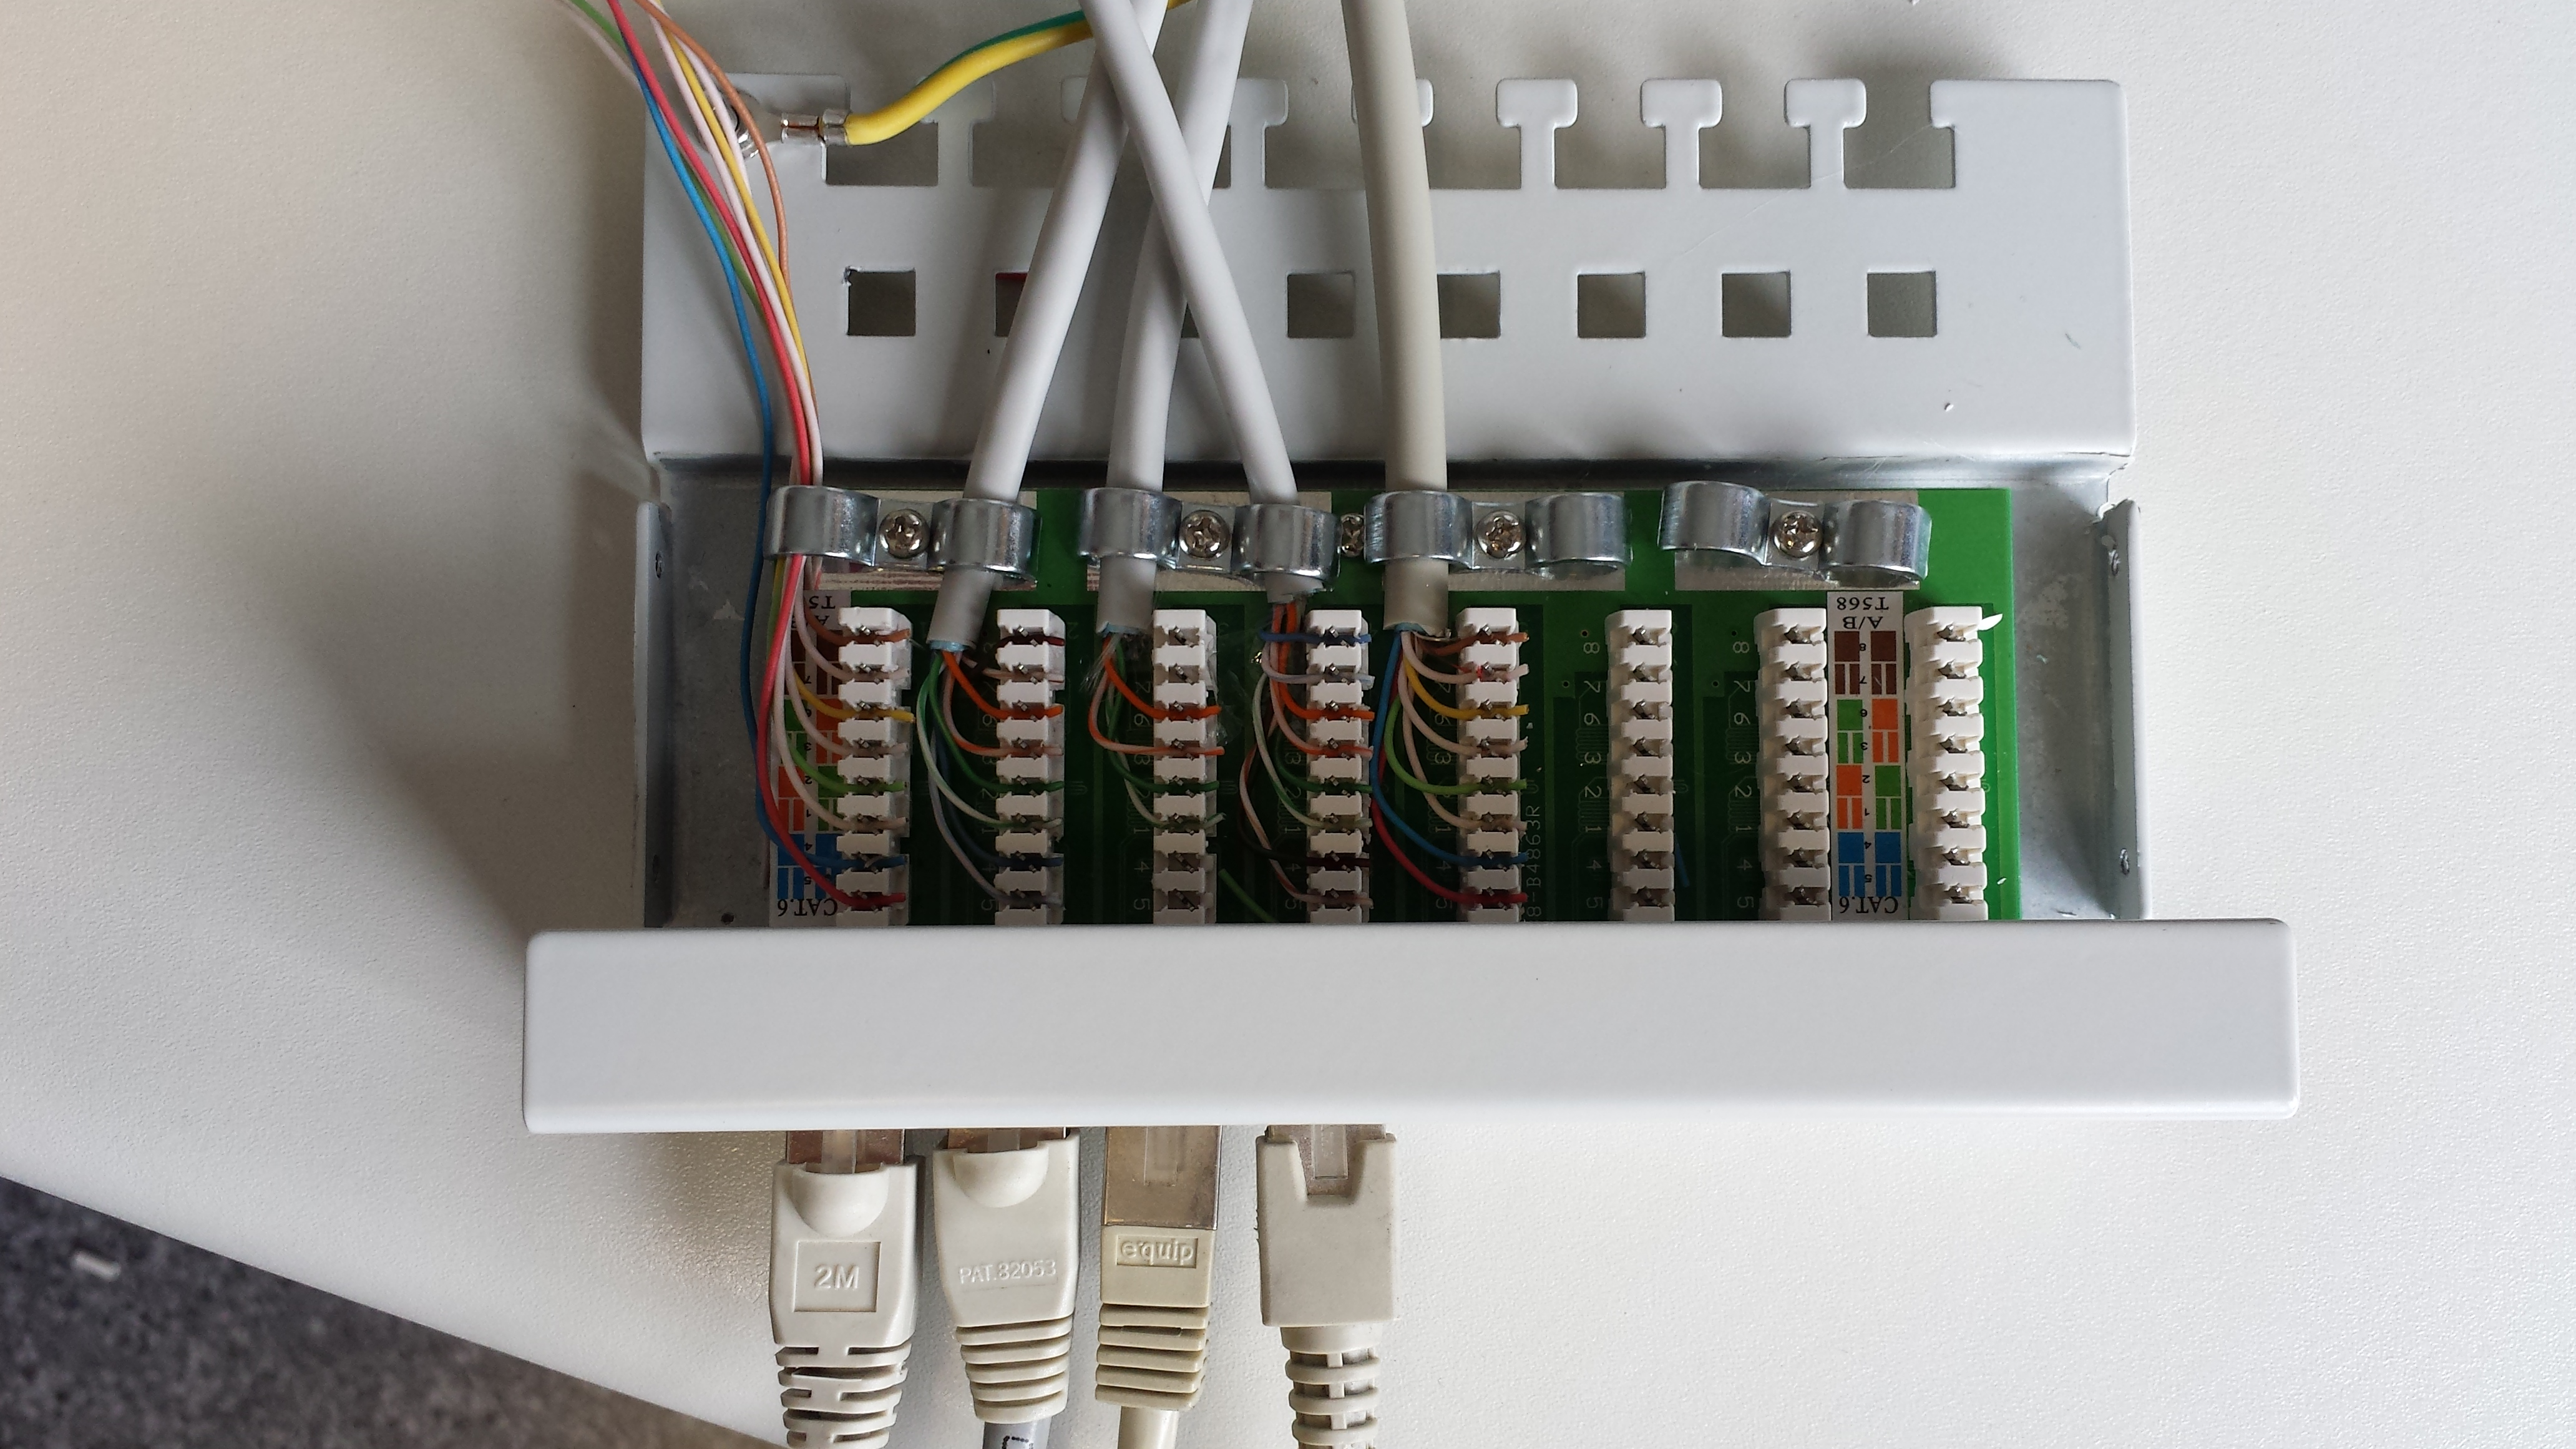
\includegraphics[width=\textwidth]{Bilder/Patchfeld1Belegung}
\caption{Belegung Patchfeld 1}\label{fig:Patch1}
\centering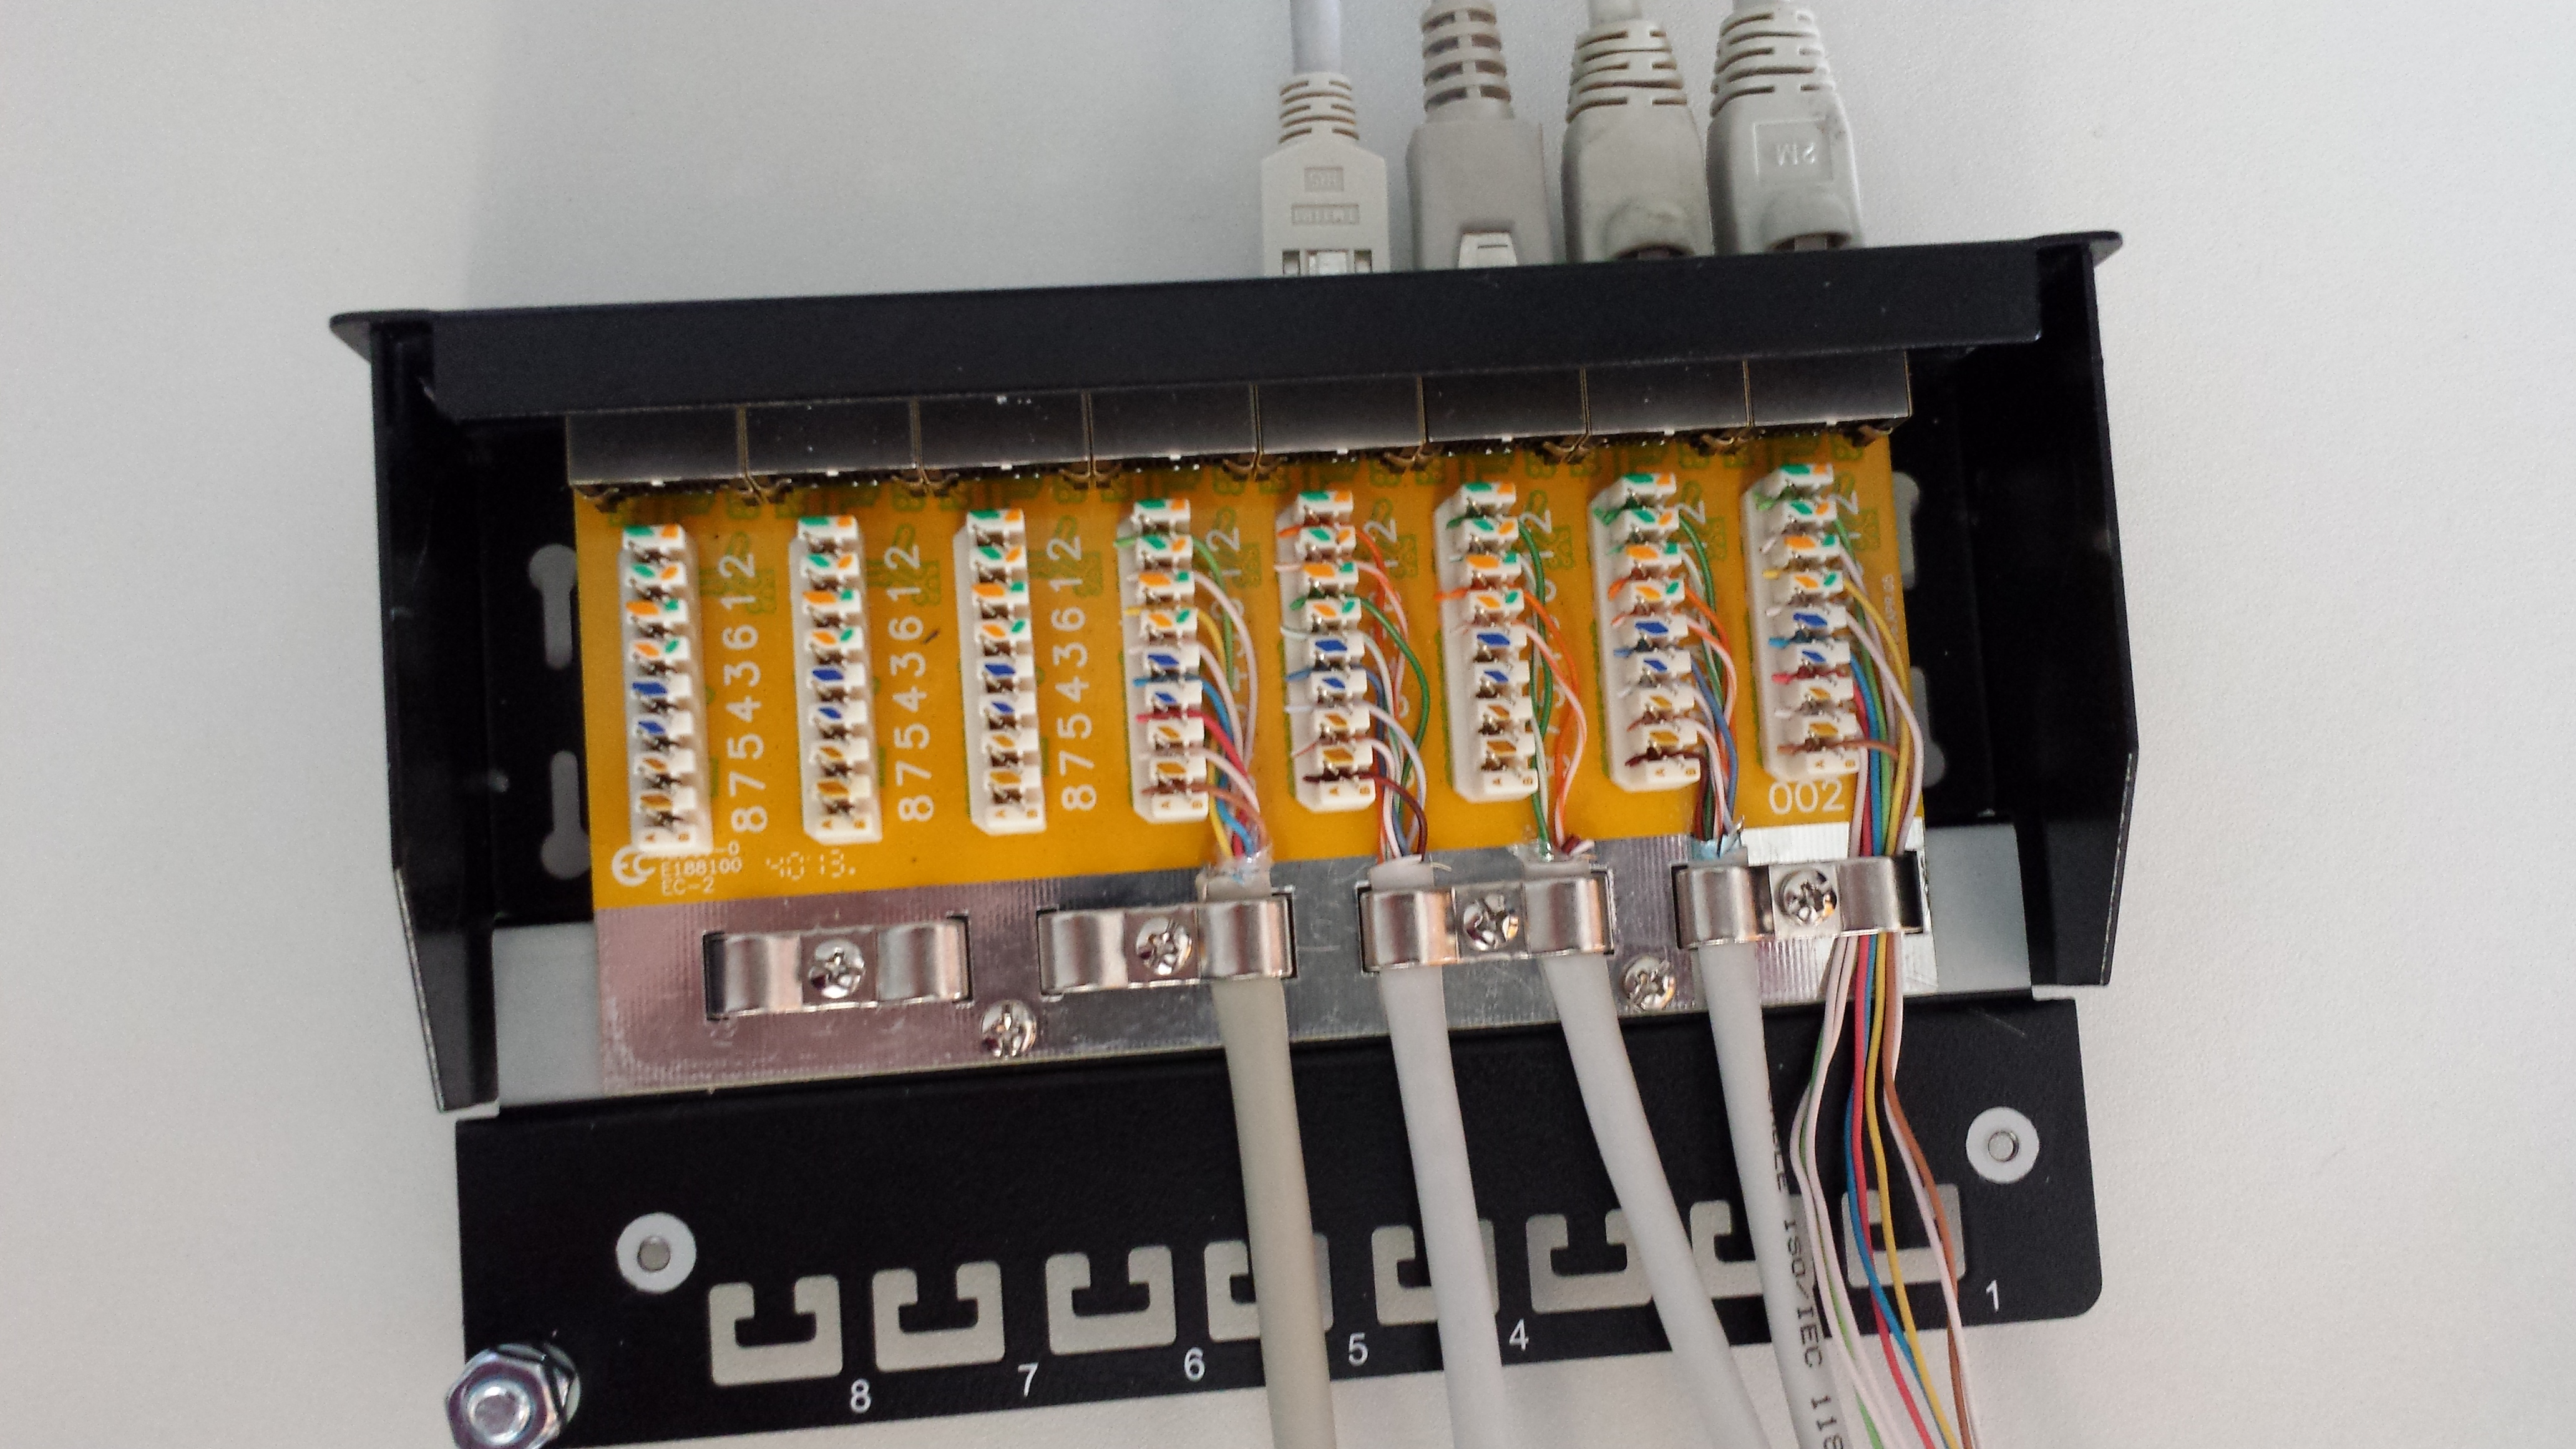
\includegraphics[angle=180,width=\textwidth]{Bilder/Patchfeld2Belegung}
\caption{Belegung Patchfeld 2}\label{fig:Patch2}
\end{figure}
(Anmerkung zu beiden Abbildungen: Port 1 ist links, das Telefonkabel in Port 1 und 5 hat vom Cat5e Standard abweichende Farben für die Kabelisolation)

(Beide Fotos \textcopyright Daniel Konrad)

\newpage
\section{Erste Messung}
Für die erste Messung haben wir auf dem Linux Fileserver eine 10.000 MiB große Datei mit binären 0 als Inhalt in der Standard SMB (Samba) Freigabe erzeugt. Der dafür verwendete Befehl war \ttfamily{dd if=/dev/zero of=10GBTestdatei bs=1M count=10000}\normalfont. Diese wurde dann auf den Windows-Clientrechnern über  den Windows Explorer kopiert und die (unter Details) angezeigte Geschwindigkeit notiert nachdem die angezeigte Datenrate sich stabilisiert hatte.

Folgende Datenraten wurden beobachtet:
\begin{itemize}
\item Port 1: 11-12 MByte/s (schwankend)
\item Port 2: 63 MByte/s
\item Port 3: 11-12 MByte/s (schwankend)
\item Port 4: 63 MByte/s
\item Port 5: 63 MByte/s
\end{itemize}
Die Datenraten von Port 1 und 3 entsprechen 100 Mbit/s.
Es konnten nicht mehr als 63 MByte/s erzielt werden da die Leserate von der Festplatte des Fileservers nur 63 MByte/s beträgt (gemessen durch ablesen der angezeigten Geschwindigkeit von\ttfamily dd if=10GBTestdatei of=/dev/null \normalfont auf dem Fileserver).

\newpage
\section{Zweite Messung}
Um testen zu können ob über Port 2, 4 und 5 eine Gigabit Verbindung möglich ist musste eine Testdatei auf einer schnelleren Datenquelle erzeugt werden. Dazu wurde auf der SMB-Freigabe des Fileservers eine neuer Ordner namens RAM erzeugt und dort eine RAM-Disk eingehängt (\ttfamily{mount -t ramfs ramfs RAM}\normalfont). auf dieser wurde dann analog zum \ttfamily{dd}\normalfont-Befehl von der ersten Messung mit \ttfamily{count=512}\normalfont eine 512 MiB große Testdatei erzeugt. Die kleinere Größe war notwendig wegen mangelnder RAM-Ausstattung des Fileservers. Die maximale Lesegeschwindkeit dieser Datei war nun 660 MByte/s (wieder gemessen durch ablesen der angezeigten Geschwindigkeit von\ttfamily dd if=Testdatei of=/dev/null \normalfont auf dem Fileserver). Mit dieser Datei wurden dann Messungen mit derselben Methode wie im ersten Versuch durchgeführt.

Es wurde nun folgende Datenraten gemessen:
\begin{itemize}
\item Port 1: 11-12 MByte/s (schwankend)
\item Port 2: 125 MByte/s
\item Port 3: 11-12 MByte/s (schwankend)
\item Port 4: 125 MByte/s
\item Port 5: 125 MByte/s
\end{itemize}
Die Datenraten von Port 1 und 3 haben sich wie zu erwarten war durch die höhere Lese-Geschwindigkeit der Datenquelle nicht verändert da schon vorher die Bandbreite der Verkabelung ausgeschöpft war. Die Ports 2, 4 und 5 erreichten nun 1 Gbit/s entsprechende Datenrate.

\end{document}
